\section{Experiments}\label{sec:experiments}

\subsection{Data and protocol}\label{sec:data}
\begin{table}[t]
\centering
\caption{Datasets. \emph{ClinVar labelled}: missense single-nucleotide variants (SNVs) with $\ge$2 review stars and a
pathogenic or likely pathogenic (P/LP) or benign or likely benign (B/LB) call, used only to put the scores on a common scale, and the number that are P/LP. \emph{Assayed}: missense
SNVs with a binary assay label outside that set, their residues and their LoF share; \emph{assayed VUS}: the subset
classified VUS in ClinVar. Shares are variant-level. Labels: the authors' classes (authors) or a rule fitted to the assay's
synonymous and nonsense controls (controls; \cref{sec:data}).}\label{tab:data}
\setlength{\tabcolsep}{4pt}
\begin{tabular}{llcrrrrrrr}
\toprule
 & & & \multicolumn{2}{c}{ClinVar labelled} & \multicolumn{3}{c}{Assayed} & \multicolumn{2}{c}{Assayed VUS}\\
\cmidrule(lr){4-5}\cmidrule(lr){6-8}\cmidrule(lr){9-10}
Gene & Assay & Labels & $n$ & P/LP & $n$ & Residues & LoF & $n$ & LoF\\
\midrule
BRCA1 & SGE \cite{Findlay2018} & authors & 345 & 156 & 1,617 & 307 & 0.161 & 272 & 0.173 \\
BRCA2 & SGE \cite{Huang2025} & controls & 309 & 94 & 3,435 & 676 & 0.130 & 704 & 0.207 \\
BAP1 & SGE \cite{Waters2024} & authors & 14 & 6 & 4,294 & 696 & 0.213 & 1,069 & 0.166 \\
RAD51C & SGE \cite{OlveraLen2024} & authors & 13 & 10 & 2,225 & 355 & 0.259 & 550 & 0.396 \\
MSH2 & DMS \cite{Jia2021} & authors & 178 & 121 & 2,906 & 893 & 0.060 & 1,542 & 0.067 \\
\midrule
Total & & & 859 & 387 & 14,477 & 2,927 & 0.164 & 4,137 & 0.167 \\
\bottomrule
\end{tabular}
\end{table}

We took every GRCh38 missense single-nucleotide variant in BRCA1, BRCA2, BAP1, RAD51C and MSH2 that is in ClinVar
\cite{Landrum2018} (release of 26 October 2026) or was assayed, annotated each on its MANE Select transcript with the
Ensembl Variant Effect Predictor \cite{McLaren2016} (AlphaMissense \cite{Cheng2023}, REVEL \cite{Ioannidis2016}) and
computed ESM-2 650M \cite{Lin2023} log-likelihood ratios by wild-type marginals \cite{Meier2021}. Labels come from five
MaveDB \cite{Esposito2019} score sets (\cref{tab:data}; accessions in \cref{s:impl}): the authors' classes for BRCA1,
BAP1 and RAD51C and the authors' threshold for MSH2 (positive loss-of-function score \cite{Jia2021}). The BRCA2 score set
has no deposited classes, so we fitted Gaussians to the assay's synonymous and nonsense variants (LoF if the posterior is
at least 0.95, functional if at most 0.05). Applied to the genes with the authors' classes, this control rule agreed on
all 1,762 BRCA1 variants confident under both, disagreed on 216 of 4,023 for BAP1 (5.4\%), and left 76.8\% of the
authors' functional RAD51C variants intermediate; \cref{sec:transfer} repeats the main experiments under these
alternative label rules. We excluded the 729 assayed variants in splice regions and set aside the
1,274 intermediate variants. One Platt map per predictor, pooled over genes, used the 859 ClinVar missense variants with
at least two review stars and a pathogenic or likely pathogenic (P/LP) or benign or likely benign (B/LB) call
(45.1\% P/LP), which are excluded from every evaluation set, leaving
14,477 assayed variants at 2,927 residues. Pooled over genes, AlphaMissense has an area under the ROC curve (AUROC) of
0.946 (95\% residue-bootstrap interval 0.922--0.965) on the ClinVar set, 0.840 (0.829--0.852) on the other assayed
variants and 0.779 (0.757--0.799) on assayed VUS. Baselines for the calls are pooled (marginal) split conformal
prediction; label-shift-weighted conformal prediction \cite{Podkopaev2021} with the true target share or its
expectation--maximization (EM) estimate \cite{Saerens2002}; fixed tiers ($q\ge0.9$ LoF, $q\le0.1$ functional); the
published AlphaMissense classes ($>0.564$, $<0.34$); and the REVEL PP3/BP4 thresholds ($\ge0.644$, $\le0.290$)
\cite{Pejaver2022}. None claims per-class coverage, and the published cut-offs target pathogenicity, so we judge them
only as assay classifiers. Coverage is residue-weighted as in $Q$; \emph{worst-class coverage} is the smaller of the mean
LoF and mean functional coverages over repetitions (\cref{fig:main}B uses the smaller of the two in each split, and
\cref{tab:mixture} in each target set). Every split is by residue (designs in \cref{tab:designs}).

\subsection{Per-class coverage and a shift in the calibration LoF share}\label{sec:coverage}
\begin{table}[t]
\centering
\caption{Per-class coverage at $\alpha=0.1$ (residue-weighted; 50 random halvings per gene). Last column: worst pair
when the calibration half is subsampled to a LoF share of 0.05 (100 halvings); fixed cut-offs use no calibration data.}\label{tab:methods}
\setlength{\tabcolsep}{4pt}
\begin{tabular}{lcccccc}
\toprule
 & & \multicolumn{3}{c}{Worst-class coverage} & & Worst pair,\\
\cmidrule(lr){3-5}
Method & Pairs & mean & worst pair & pairs $<0.85$ & Abstention & share 0.05\\
\midrule
Per-class (ours) & 15 & 0.901 & 0.896 & 0 & 0.35 & 0.899 \\
Pooled conformal & 15 & 0.836 & 0.545 & 5 & 0.42 & 0.113 \\
Label-shift weighted, true share & 15 & 0.836 & 0.559 & 5 & 0.42 & 0.598 \\
Label-shift weighted, EM share & 15 & 0.722 & 0.039 & 9 & 0.36 & 0.038 \\
Fixed tiers ($q\ge0.9$, $q\le0.1$) & 15 & 0.871 & 0.663 & 5 & 0.53 & -- \\
AlphaMissense classes & 5 & 0.725 & 0.540 & 4 & 0.11 & -- \\
REVEL PP3/BP4 thresholds & 5 & 0.700 & 0.445 & 5 & 0.42 & -- \\
\bottomrule
\end{tabular}
\end{table}

Over 50 random halvings of each gene's residues (calibrate on one half, test on the other), the in-expectation rule at
$\alpha=0.1$ gave worst-class coverage between 0.896 and 0.908 in all 15 gene--predictor pairs, none more than one Monte
Carlo standard error (0.002--0.010) below the target (\cref{tab:methods}, \cref{fig:main}A; per pair in
\cref{tab:main}). Pooled conformal fell to 0.545 on LoF variants and below 0.85 in 5 pairs, because a marginal threshold
controls coverage averaged over the two classes, not within each (in MSH2, with 6\% LoF variants, it was the functional
class that fell marginally below 0.90); the published cut-offs covered functional variants as little as 0.540
(AlphaMissense, BAP1) and 0.445 (REVEL, MSH2). The per-class rule abstained on 35\% of variants on average (17--47\%),
against 42\% for pooled conformal and 11\% for the AlphaMissense classes. Calibrating on all variants of the calibration
half instead of one per residue used about five times as many labels and abstained less (30.4\% against 35.5\%); but in
a separate run of 50 halvings that compared the two, worst-class coverage fell below 0.90 in 12 of 15 pairs (lowest
0.885), against 5 (lowest 0.897) for one variant per residue. All-variant calibration weights variants while the test weights residues; weighting each
residue equally left 1 pair below 0.90 (lowest 0.898) but abstained more (44.6\%), which points to the weighting
rather than the dependence, so we keep one variant per residue.

To compare the methods under a prevalence shift, we subsampled each calibration half to a LoF share of 0.05 to 0.5 and
tested at the natural share (100 repetitions; \cref{fig:shift}A). Subsampling by class leaves each class's score law
unchanged, so Corollary~\ref{cor:shift} predicts the per-class result; the question is what happens to the
baselines. The per-class rule kept worst-class
coverage between 0.897 and 0.925 in every pair at every share (0.891--0.925 in a separate run balanced at 50\% LoF),
with abstention rising from 37\% to 83\% as LoF variants became scarce. Pooled conformal calibrated at share 0.05
covered LoF variants at 0.113 in its worst pair, and label-shift-weighted conformal fell to 0.53--0.60 with the true
target share and to 0.04 with the EM estimate, which missed the LoF share by 0.255 on average because ClinVar
pathogenicity and assay loss of function differ in definition as well as in class share.

\begin{figure}[t]
\centering
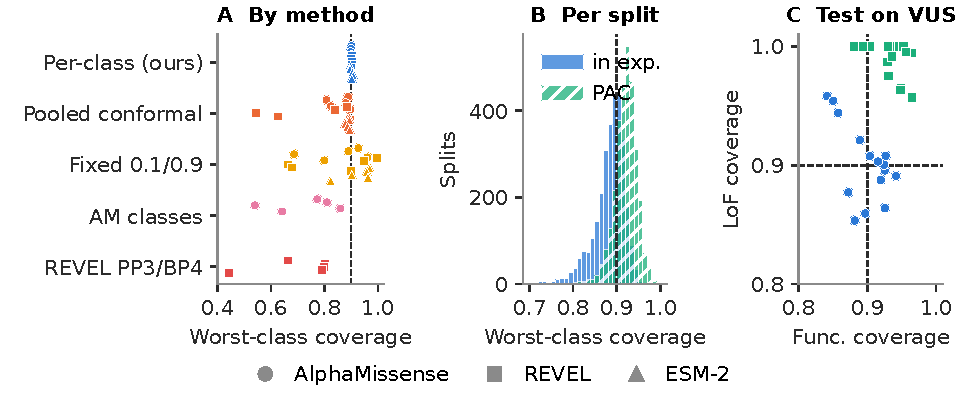
\includegraphics[width=\linewidth]{fig_main.pdf}
\caption{Per-class coverage at $\alpha=0.1$. Marker shape: predictor (panels A, C); colour and line style: threshold
rule (panels B, C). (A) Worst-class coverage for each gene--predictor pair (50 splits); AlphaMissense cl.: the published
AlphaMissense classes. (B) Smaller of the two per-class coverages in each test half, pooled over pairs (3,000 splits per
rule). (C) Coverage on assayed VUS with thresholds set on non-VUS variants at other residues (50
repetitions).}\label{fig:main}
\end{figure}

\subsection{Reliability across splits and a real change of population}\label{sec:shift}
With 17 to 93 LoF residues per calibration half, a single split can miss the in-expectation guarantee: over 200 splits
per pair, LoF coverage on the test half was below 0.90 in 36.4\% of splits and functional coverage in 43.6\%
(\cref{fig:main}B). PAC thresholds ($\delta_{\mathrm P}=0.1$) reduced these to 7.9\% and 10.8\% at the price of
abstaining on 58.4\% of variants against 35.4\%. A finite test half adds sampling noise to the coverage that
Propositions~\ref{prop:mondrian} and~\ref{prop:pac} bound. Computed exactly on all of a gene's residues for calibration
samples drawn from them (200 draws per pair), PAC coverage fell below 0.90 in 4.8\% (LoF) and 7.1\% (functional) of
draws and in at most 10.0\% in any pair, within $\delta_{\mathrm P}$; in-expectation coverage did so in 34.3\% and
42.9\%. Calibrated on non-VUS variants of one half of each gene's residues and applied to the assayed VUS of the other
half (residue-weighted LoF share 17.0\% in the calibration sample and 19.8\% among the VUS), in-expectation thresholds
kept LoF coverage between 0.854 and 0.958 and functional coverage between 0.841 and 0.942, each below 0.90 in 7 of 15
pairs (\cref{fig:main}C); PAC thresholds kept LoF coverage at or above 0.957, but functional coverage fell below 0.90 in 2
of 15 pairs (lowest 0.881), and they abstained on 81.7\% of VUS; on VUS, Assumption~\ref{as:shift} holds only
approximately.

\subsection{Certified likelihood ratios}\label{sec:evidence}
\begin{table}[t]
\centering
\caption{Threshold selection judged against the population likelihood ratio (oracle design, grid $G_4$, $\delta=0.05$,
1,500 draws; all rules on the same draws). Guarantee: finite-sample validity after selection, for every level of a call
type at once or for each level separately. Bounds held: draws in which every claimed bound was respected (fixed-sequence
rules certify a level, not a bound; a point estimate is not a bound). Levels held: draws in which every claimed level
held. Last four columns: share of draws certifying each level (\%); no rule with a guarantee certified a strong level.}
\label{tab:oracle}
\setlength{\tabcolsep}{3.4pt}
\begin{tabular}{llcccccc}
\toprule
 & Finite-sample & Bounds & Levels & \multicolumn{2}{c}{LoF calls} & \multicolumn{2}{c}{Functional calls}\\
\cmidrule(lr){5-6}\cmidrule(lr){7-8}
Selection rule & guarantee & held & held & supp. & mod. & supp. & mod.\\
\midrule
Certified (ours), Bonferroni & yes, all levels & 99.7 & 99.9 & 86.7 & 13.3 & 44.9 & 1.5 \\
Certified (ours), fixed sequence & yes, all levels & -- & 99.9 & 74.9 & 14.4 & 43.8 & 1.5 \\
Fixed sequence, each level at $\delta$ & yes, per level & -- & 99.7 & 87.2 & 30.5 & 61.9 & 3.9 \\
Clopper--Pearson, uncorrected & no & 97.9 & 99.5 & 95.9 & 35.1 & 68.0 & 6.9 \\
Katz interval, Bonferroni & no & 98.0 & 99.7 & 99.3 & 52.5 & 52.4 & 0.2 \\
Percentile bootstrap & no & 57.6 & 72.5 & 99.9 & 78.1 & 90.0 & 45.1 \\
Percentile bootstrap, Bonferroni & no & 65.3 & 75.1 & 98.1 & 52.3 & 74.3 & 36.8 \\
Percentile bootstrap, $+0.5$ counts & no & 75.4 & 88.2 & 99.9 & 76.6 & 89.3 & 37.3 \\
Point estimate & no & 15.5 & 42.1 & 100.0 & 98.2 & 99.8 & 75.7 \\
\bottomrule
\end{tabular}
\end{table}

Treating each gene's assayed residues as the population, we drew calibration (30\%) and certification (50\%) residues
with replacement, 100 times per pair, ran \cref{alg:certivar} with $\delta=0.05$ on the four-point grid
$G_4=\{0.05,0.10,0.20,0.30\}$, and
computed the population likelihood ratio of every selection exactly. All rules were applied to the same draws
(\cref{tab:oracle}). Because Assumption~\ref{as:cluster} holds here by construction, this design checks the
certificates' arithmetic and the competitors' failures; the held-out regions of \cref{sec:transfer} test what happens
when it does not. Every bound claimed in a draw was respected in 99.7\% of the 1,500 draws for the certified rule
(Theorem~\ref{thm:lr} guarantees at least 90\%). Percentile-bootstrap bounds were all respected in only 57.6\% of draws,
65.3\% with a Bonferroni correction and 75.4\% with 0.5 added to every count; 59\% of bootstrap failures came from
certification samples with no false call of that type, where the bound failed 89\% of the time. Point estimates claimed
levels that all held in only 42.1\% of draws; their strong LoF claims held in 50 of 235 (\cref{fig:evidence}). Two
rules without a guarantee after selection, uncorrected Clopper--Pearson bounds and Katz intervals with a Bonferroni
correction, held in 97.9\% and 98.0\% of draws and certified more often (Clopper--Pearson at every level, Katz at three
of the four): Katz bounds reached LoF-moderate in 52.5\% of draws against 13.3\%. The exact certificate therefore costs yield, which buys a
guarantee that holds at every sample size.

\textsc{CertiVar} certified LoF-supporting calls in 86.7\% of draws (calling 25.2\% of variants), functional-supporting
calls in 44.9\% (61.4\% called), LoF-moderate in 13.3\% and functional-moderate in 1.5\%, and never a strong level.
Per-class coverage at the selected $\alpha$ averaged 0.81 (LoF) and 0.80 (functional), above the guaranteed 0.70
(Proposition~\ref{prop:select}): selecting for evidence strength trades coverage for confidence. Claimed levels held in
99.9\% of certified claims when the likelihood ratio was weighted by variant rather than by residue. Fixed-sequence
testing with the level-simultaneous guarantee of Theorem~\ref{thm:fs}(b) traded supporting for moderate evidence: on
$G_4$ it certified LoF-moderate in 14.4\% of draws against 13.3\% but LoF-supporting in 74.9\% against 86.7\%, and on a
20-point grid ($G_{20}$, 20 equally spaced values from 0.02 to 0.40) LoF-moderate in 12.7\% against 6.4\% but
LoF-supporting in 50.3\% against 74.8\% (\cref{fig:shift}B). Testing each level at the full $\delta$, which guarantees one
level at a time, reached LoF-moderate in 30.5\% of draws on $G_4$; the testing order also matters, since functional
levels tested in increasing $\alpha$ reached functional-supporting in 24.7\% of draws against 61.9\%. On held-out fifths
of the residues, empirical likelihood ratios respected the certified bounds in 98.7\% of 2,091 cases (bootstrap:
76.8\%); on VUS at other residues, LoF-supporting held in all 443 certified claims and LoF-moderate in 25 of 28.
Against ClinVar labels (exploratory, not independent of the assays), LoF calls had likelihood-ratio lower bounds of
4.9--19.6 (BRCA1), 7.6--9.4 (BRCA2) and 2.6--3.2 (MSH2) (\cref{tab:app_clinvar}).

\begin{figure}[t]
\centering
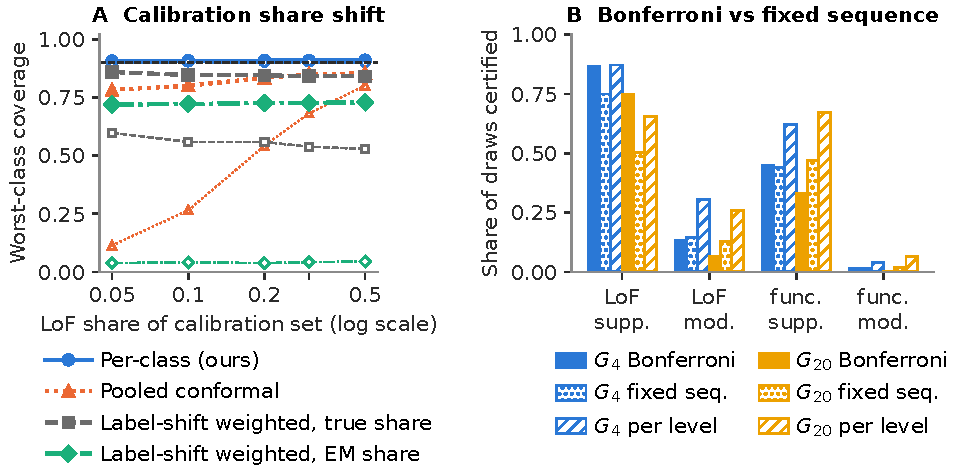
\includegraphics[width=\linewidth]{fig_shift.pdf}
\caption{(A) Worst-class coverage when the calibration half is subsampled to a given LoF share (0.05, 0.1, 0.2, 0.3 and
0.5, log scale): mean over 15 pairs (thick) and worst pair (thin, open markers). (B) Share of oracle draws certifying each
level with a Bonferroni correction, with fixed-sequence testing simultaneous over levels (fixed seq.), or with
fixed-sequence testing of each level at the full $\delta$ (per level), on the four-point ($G_4$) and 20-point
($G_{20}$) grids.}\label{fig:shift}
\end{figure}

\subsection{Checking invariance, and where CertiVar applies}\label{sec:check}
\begin{table}[t]
\centering
\caption{Mixture-consistency check ($p<0.05$; one target variant per residue). Coverage: mean over target sets of the
smaller per-class coverage in each set (a per-set measure, unlike \cref{tab:methods}) of in-expectation thresholds
($\alpha=0.1$) set on the same calibration data.}\label{tab:mixture}
\setlength{\tabcolsep}{4pt}
\begin{tabular}{llcccc}
\toprule
 & & Target & Rejected & \multicolumn{2}{c}{Worst-class coverage}\\
\cmidrule(lr){5-6}
Target set & Assumption~\ref{as:shift} & sets & (\%) & accepted & rejected\\
\midrule
Random half of the residues & holds by design & 1,500 & 4.7 & 0.880 & 0.880 \\
Assayed VUS at other residues & approximately & 750 & 8.5 & 0.845 & 0.816 \\
Held-out contiguous quarter & not assumed & 1,500 & 43.9 & 0.837 & 0.788 \\
Another gene's calibration data & not assumed & 300 & 77.3 & 0.745 & 0.644 \\
Unassayed VUS, other residues & unknown (no labels) & 120 & 100.0 & -- & -- \\
\bottomrule
\end{tabular}
\end{table}

The mixture-consistency check of \cref{sec:method} rejected 4.7\% of random halves (3.0--7.7\% by gene), where
Assumption~\ref{as:shift} holds by design, so it keeps close to its 5\% level (\cref{tab:mixture}). It rejected 43.9\% of held-out contiguous quarters,
77.3\% of transfers from another gene's calibration data and every set of unassayed ClinVar VUS at residues the BRCA1
and BRCA2 assays did not reach; on those VUS the thresholds abstained on only 8.9\% of variants (mean over predictors
and the two genes), against 35\% on assayed residues. Where labels exist, rejected targets had lower coverage than
accepted ones (0.788 against 0.837 for quarters, 0.644 against 0.745 across genes). The check has little power for
assayed VUS (8.5\% rejected), whose accepted sets had a mean worst-class coverage of 0.845 against 0.880 for random
halves on the same measure, so passing it is not evidence that the guarantees transfer. Across the five genes, 147
ClinVar missense VUS were unassayed but lay at assayed residues, 105 of them in MSH2 (\cref{tab:app_usecase,tab:app_usecase_calls}). Even
these need not be exchangeable with the assayed variants, since they are the ones the assay missed: for MSH2 the check
rejected 40\% of samples with AlphaMissense and 35\% with REVEL, but none with ESM-2, whose thresholds gave certified
LoF-supporting calls to 19.1 and functional-supporting calls to 5.0 of the 105 on average over 20 splits; for the other
two predictors, \cref{tab:app_usecase_calls} averages only over the splits the check accepted. Of the 4,044 unassayed VUS at other residues, the 4,010 in BRCA1 and BRCA2 are not called,
because the check rejected every sample of them; the other 34 are too few to check.

\subsection{How much data, from where, and with which labels}\label{sec:transfer}
Calibration data had to come from the same gene: calibrating on the other four genes left 8 of 15 pairs below 0.85
(worst 0.487), consistent with gene-specific evidence strength \cite{Tejura2024,Chen2026}. Calibrating on three
contiguous quarters of a protein and testing on the fourth gave worst-class coverage of 0.860--0.923, and 88.8\% of 1,891
certified bounds held against the empirical likelihood ratios of the held-out quarter, below the 95\% that Theorem~\ref{thm:lr}
guarantees under Assumption~\ref{as:cluster} (those ratios carry their own sampling noise). With 150 calibration residues drawn at random, coverage
averaged over genes met the target with 40.5\% abstention (worst pair 0.890; 82.8\% abstention with 25 residues).
Coverage was lower on the third of variants nearest the assay class boundary (0.865 LoF, 0.873 functional).
Intermediate variants, which no guarantee covers, were called LoF in 19.6\% and functional in 36.6\% of cases.
Relabelling BRCA2, BAP1 and RAD51C with alternative rules (\cref{tab:app_labels}) changed yields but not validity: the
lowest per-class coverage over predictors stayed between 0.894 and 0.902, and certified bounds held in 2,530 of 2,533
oracle selections.
